%-----------------------------------------------------------------------------%
\chapter{\babDua}
%-----------------------------------------------------------------------------%

%-----------------------------------------------------------------------------%
\section{Kajian Penelitian Terkait}
%-----------------------------------------------------------------------------%
Banyak sekali referensi yang menjadi bagian besar dalam tertulisnya proposal ini, referensi tersebut terdiri atas berbagai macam jenis literatur dari sumber yang dapat diakses secara daring. Tak sedikit pula literatur tersebut menjadi alasan besar latar belakang dari proposal ini dilahirkan, berikut adalah beberapa penelitian terdahulu yang menjadi referensi dalam melakukan penyusunan proposal ini :

% Penelitian Terdahulu
\begin{center}
	\newcolumntype{L}[1]{>{\raggedright\let\newline\\\arraybackslash\hspace{1pt}}m{#1}}
	\newcolumntype{C}[1]{>{\centering\let\newline\\\arraybackslash\hspace{1pt}}m{#1}}
	\newcolumntype{R}[1]{>{\raggedleft\let\newline\\\arraybackslash\hspace{1pt}}m{#1}}
	
	\begin{longtable}{|>{\centering\arraybackslash}p{0.6cm}|p{4cm}|p{4cm}|p{4cm}|}
	\caption{Penelitian Terdahulu}
	\label{tab:PenelitianDulu}\\
	
	\hline
	\textbf{No.} & \textbf{Judul} & \textbf{Penulis} & \textbf{Hasil}\\
	\hline
	
	1.& \textit{Multitarget Physical Activities Monitoring and Classification Using a V-Band FMCW Radar} (2023)
	& Rizzi Varela, Victor G.; Rodrigues, Davi V. Q.; Zeng, Leya; Li, Changzhi
	& - \\ \hline
	
	2. & \textit{A Short-Range FMCW Radar-Based Approach for Multi-Target Human-Vehicle Detection} (2022)
	& Tavanti, Emanuele; Rizik, Ali; Fedeli, Alessandro; Caviglia, Daniele D.; Randazzo, Andrea 
	& - \\ \hline
	
	3. & \textit{FMCW Radar With Enhanced Resolution and Processing Time by Beam Switching} (2021)
	& Hilario Re, Pascual D.; Comite, Davide; Podilchak, Symon K.; Alistarh, Cristian A.; Goussetis, George; Sellathurai, Mathini; Thompson, John; Lee, Jaesup
	& - \\ \hline
	
	4. & \textit{An X–band FMCW Radar Demonstrator Based on an SDR Platform} (2020)
	& Dabrowski, Grzegorz; Stasiak, Krzysztof; Drozdowicz, Jedrzej; Gromek, Damian; Samczynski, Piotr
	& - \\ \hline
	
	5. & \textit{Single Target Recognition Using a Low-Cost FMCW Radar Based on Spectrum Analysis} (2020)
	& Rizik, Ali; Tavanti, Emanuele; Vio, Roberto; Delucchi, Alessandro; Chible, Hussien; Randazzo, Andrea; Caviglia, Daniele D.
	& - \\ \hline
	
	6. & \textit{Educational Low-Cost C-Band FMCW Radar System Comprising Commercial Off-the-Shelf Components for Indoor Through-Wall Object Detection} (2021)
	& Jeong, Hyunmin; Kim, Sangkil
	& - \\ \hline
	
	7. & \textit{Modified FMCW system for non-contact sensing of human respiration} (2020)
	& Pramudita, Aloysius Adya; Suratman, Fiky Y.; Arseno, Dharu
	& - \\ \hline
	
	8. & \textit{FMCW Radar for Noncontact Bridge Structure Displacement Estimation} (2023)
	& Pramudita, Aloysius Adya; Lin, Ding-Bing; Dhiyani, Azizka Ayu; Ryanu, Harfan Hian; Adiprabowo, Tjahjo; Yudha, Erfansyah Ali
	& - \\ \hline
	
	9. & \textit{A Novel Scheme of High-Precision Heart Rate Detection With a mm-Wave FMCW Radar} (2023)
	& Zhou, Min; Liu, Yunxue; Wu, Shie; Wang, Chengyou; Chen, Zekun; Li, Hongfei
	& - \\ \hline
	\end{longtable}
\end{center}
%-----------------------------------------------------------------------------%
%\section{Teori Dasar}
%-----------------------------------------------------------------------------%

\section{Radar}

Penggunaan gelombang elektromagnetik sebagai sarana untuk mendeteksi objek adalah konsep dasar dari radar. Radar sendiri merupakan singkatan dari \textit{Radio Detection and Ranging}, dari situ sangat nampak sekali tujuan dari penggunaan alat ini, yaitu untuk mendeteksi sesuatu dan mengukur jarak dengan menggunakan gelombang radio. 

Cara kerja dari radar adalah dengan memancarkan gelombang di dalam ruang bebas yang kemudian radar akan mendeteksi gelombang pantulan dari objek tersebut. Adanya gelombang yang terpantul ini tidak hanya menunjukkan keberadaan dari suatu objek, namun dengan membandingkan gelombang pantulan yang diterima dengan gelombang yang dikirimkan maka informasi tentang objek yang terdeteksi dapat didapat \cite{Skolnik2001}.

\begin{equation}
	R = \frac{cT_{R}}{2}
	\label{eq:PersRadar}
\end{equation}

Persamaan \ref{eq:PersRadar} menjelaskan jarak antara target dengan antena, dengan $T_{R}$ sebagai waktu sinyal radar bergerak secara bolak balik dari dan menuju objek. Karena radar memakai gelombang elektromagnetik, maka $c$ memiliki kecepatan yang sama dengan cahaya, yaitu $3 \times 10 ^{8}$.

Pada gambar \ref{pic:skemaRadar} berikut, skema dan konsep dasar dari cara kerja radar dapat diamati. Terlihat bahwa sinyal yang dikirimkan akan mengenai target, dalam kasus ini adalah pesawat, lalu sinyal yang mengenai objek akan kembali dengan sinyal yang lebih kecil dengan amplitudo yang lebih rendah. Perubahan pada gelombang yang terpantul dapat menggambarkan perilaku yang sedang ditunjukkan oleh objek yang di deteksi, mulai dari pengurangan amplitudo hingga pergeseran fasa.

\begin{figure}
	\begin{center}
		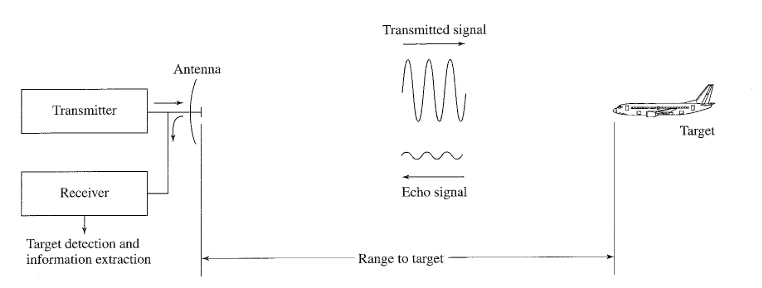
\includegraphics[scale=0.5]{pics/bab2/skemaradar.png} 
		\caption[Skema Dasar Radar]{{Skema Dasar Radar} \cite{Skolnik2001}}
		\label{pic:skemaRadar}
	\end{center}
\end{figure}

Gambar \ref{pic:blokdiagram} menunjukkan blok diagram dari sistem radar pulsa sederhana. Dapat dilihat beberapa komponen yang membentuk seluruh sistem radar, semua komponen ini memiliki perannya sendiri sehingga proses pengiriman dan pendeteksian sinyal dapat dilakukan.  Bila seluruh sistem bekerja dengan baik, maka proses yang ditunjukkan pada penjelasan skema dasar radar dapat berjalan dengan lancar.

\begin{figure}
	\begin{center}
		\includegraphics[scale=0.35]{pics/bab2/blokdiagram.png} 
		\caption[Blok Diagram Radar]{{Blok Diagram Radar Sederhana \cite{Kingsley1999}}}
		\label{pic:blokdiagram}
	\end{center}
\end{figure}

Persamaan radar berguna untuk menghubungkan seluruh komponen yang terdapat pada suatu sistem radar. Hubungan di antara seluruh komponen tersebut akan di perlihatkan secara matematis, sehingga penerapannya pada suatu alat akan terlihat dengan jelas. Dengan adanya beberapa persamaan ini, proses desain suatu radar akan menjadi lebih mudah dilakukan dan prediksi dari hasil radar yang dirancang bisa didapatkan.

Salah satu persamaan pada radar adalah \textit{maximum unambiguous range}, yang bersimbol $R_{un}$, dengan $T_{p}$ sebagai periode pengulangan pulsa, yang bernilai $\frac{1}{f_{p}}$, dengan $f_{p}$ sebagai frekuensi pengulangan pulsa.

\begin{equation}
	R_{un} = \frac{cT_{p}}{2} = \frac{c}{2f_{p}}
\end{equation}

Bila antena yang digunakan dalam memancarkan gelombang elektromagnetika radar bersifat isotrop, maka kerapatan daya pada jarak $R$ dari radar akan sama dengan daya di transmisi ($P_{t}$) dibagi luas permukaan $4\pi R^{2}$ dari sebuah bola imajiner dengan radius $R$, atau dapat didefinisikan pula dengan.

\begin{equation}
	P = \frac{P_{t}}{4\pi R^{2}}
\end{equation}

Namun, pada kenyataannya radar seringkali menggunakan antena \textit{directive} untuk mengkonsentrasikan daya yang terradiasi pada arah tertentu. Maka kerapatan dayanya adalah

\begin{equation}
	\text{Kerapatan daya antena \textit{directional}} = \frac{P_{t} G}{4\pi R^{2}}
\end{equation}

Dengan G sebagai \textit{gain} maksimum suatu antena, yaitu

\begin{equation}
	G  = \frac{\text{Kerapatan daya maksimum dari antena \textit{directional}}}{\text{Kerapatan daya antena Isotrop \textit{lossless} dengan daya yang sama}}
\end{equation}

\textit{Radar Cross Section} atau yang sering disingkat dengan RCS merupakan daerah suatu objek dari target yang dapat terdeteksi oleh suatu radar. Area tersebut diperhitungkan dengan mempertimbangkan bentuk dari objek dan interaksinya dengan gelombang elektromagnetik. Pada \ref{pic:RCS} ditunjukkan beberapa sifat RCS dan persamaannya.

\begin{center}
	\begin{figure}[h!]
		\begin{subfigure}[b]{0.5\linewidth}
			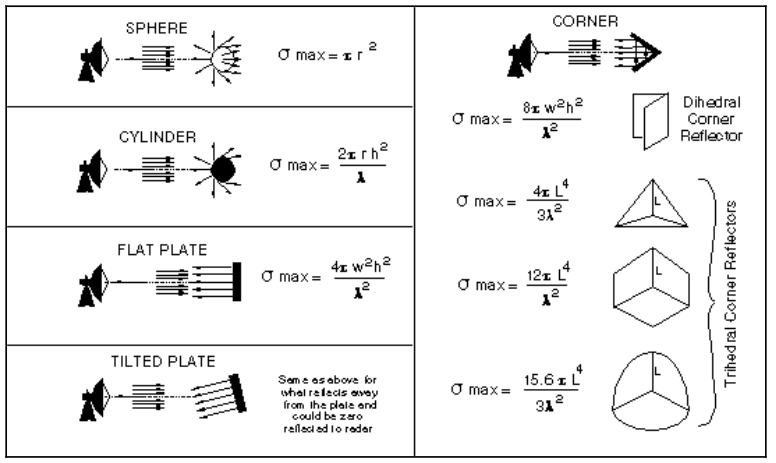
\includegraphics[width=\linewidth]{pics/bab2/rcsBentuk.png}
			\caption{Bentuk dan Persamaan \textit{Radar Cross Section}}
		\end{subfigure}
		\begin{subfigure}[b]{0.5\linewidth}
			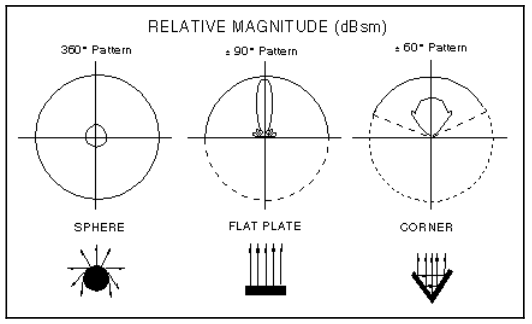
\includegraphics[width=\linewidth]{pics/bab2/rcsPola.png}
			\caption{Pola Radiasi dari \textit{Radar Cross Section}}
		\end{subfigure}
		\caption[\textit{Radar Cross Section}]{\textit{Radar Cross Section} \cite{ONeill2012}}
		\label{pic:RCS}
	\end{figure}
\end{center}

\section{Pengolahan Sinyal Radar}
Untuk mendapat suatu kesimpulan dari sinyal radar, maka dibutuhkan pengolahan sinyal radar yang tepat. Pengolahan sinyal tersebut dilakukan mulai dari pembentukan gelombang hingga pengambilan kesimpulan. 

\subsection{Bentuk Gelombang Radar}
\begin{figure}
	\begin{center}
		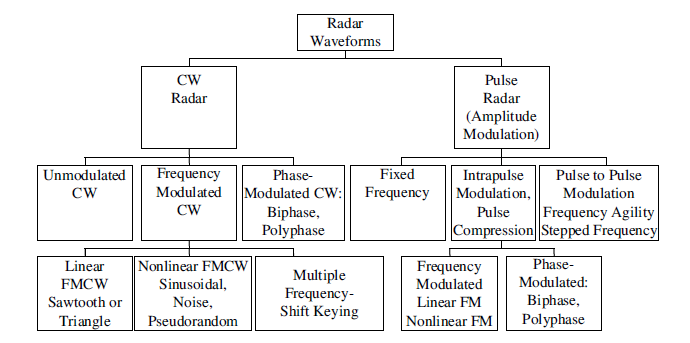
\includegraphics[scale=0.8]{pics/bab2/radarwaveform.png}
		\caption[Bentuk Gelombang Radar]{Bentuk Gelombang Radar \cite{Melvin2014}}
		\label{pic:bentukgelradar}
	\end{center}
\end{figure}
Bentuk gelombang radar dapat dibedakan menjadi dua kelas, yaitu radar dengan gelombang kontinyu dan radar pulsa. Seperti pada gambar \ref{pic:bentukgelradar}, kedua kelas tersebut masih dapat dibagi lagi kedalam beberapa teknik lain. Penggunaan salah satu jenis gelombang ditentukan berdasarkan kebutuhan radar yang akan di desain. 

Radar dengan gelombang pulsa akan memancarkan gelombang elektromagnetik dalam waktu singkat lalu jeda sejenak sesuai waktu yang ditentukan. Pada waktu jeda tersebut, radar akan mendeteksi sinyal pantul dari gelombang yang dikirim sebelumnya. Setelah waktu jeda berakhir, radar akan kembali memancarkan gelombang pulsa lagi. Radar dengan gelombang ini akan memancarkan gelombang elektromagnetik dengan \textit{power} yang tinggi. 

Sedangkan radar dengan gelombang kontinyu akan terus memancarkan serta menerima gelombang elektromagnetik tanpa henti dalam waktu yang bersamaan. Sehingga radar dengan gelombang kontinyu hanya digunakan pada sistem dengan \textit{power} yang rendah dengan jarak maksimum deteksi yang kecil. Hal ini disebabkan karena sering terjadinya kebocoran dari antena pengirim ke antena penerima. Alasan ini pula yang mendasari keputusan penggunaan \textit{power} yang rendah \cite{Scheer2015}.

\subsection{\textit{Frequency Modulated Continuous Wave Radar}}

Radar FMCW memancarkan sinyal yang bila terpantul objek, akan kembali terdeteksi. Hal ini dapat direalisasikan dengan blok diragram dari sistem radar FMCW seperti pada gambar \ref{pic:FMCWBlock}.  

\begin{figure}
	\begin{center}
		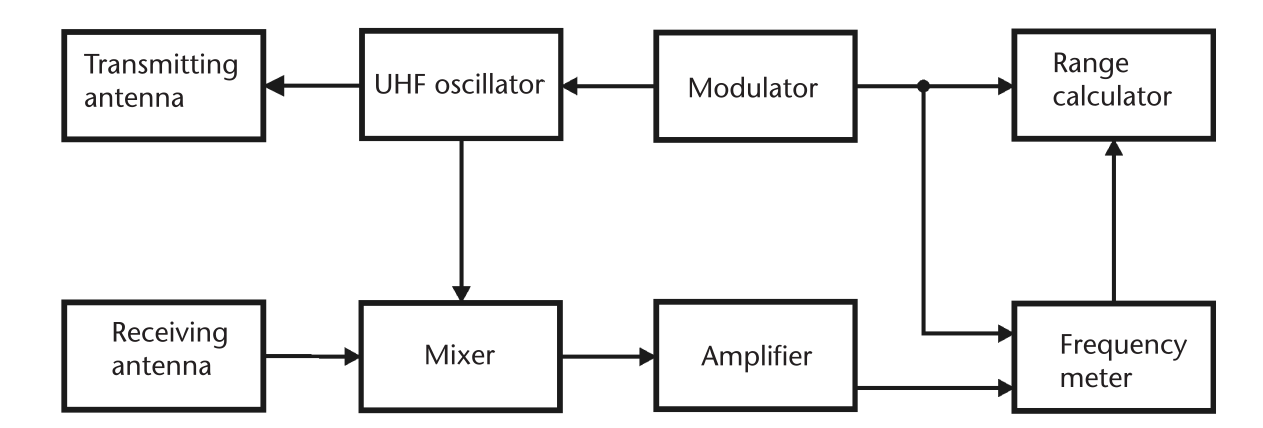
\includegraphics[scale=0.3]{pics/bab2/blokDiagramFMCW.png}
		\caption[Blok Diagram Radar FMCW]{Blok Diagram Radar FMCW}
		\label{pic:FMCWBlock}
	\end{center}
\end{figure}

Dari blok diagram tersebut, dapat dilihat bahwa sinyal yang diterima dicampurkan dengan sinyal yang dikirim, sehingga karena adanya \textit{delay} yang disebabkan oleh jarak gelombang bergerak, maka akan terdeteksi perbedaan frekuensi. Dengan begitu, perbedaan pada fasa dan frekuensi menjadi tolok ukur antara sinyal yang dikirim dengan sinyal yang di dapatkan kembali.

\begin{figure}
	\begin{center}
		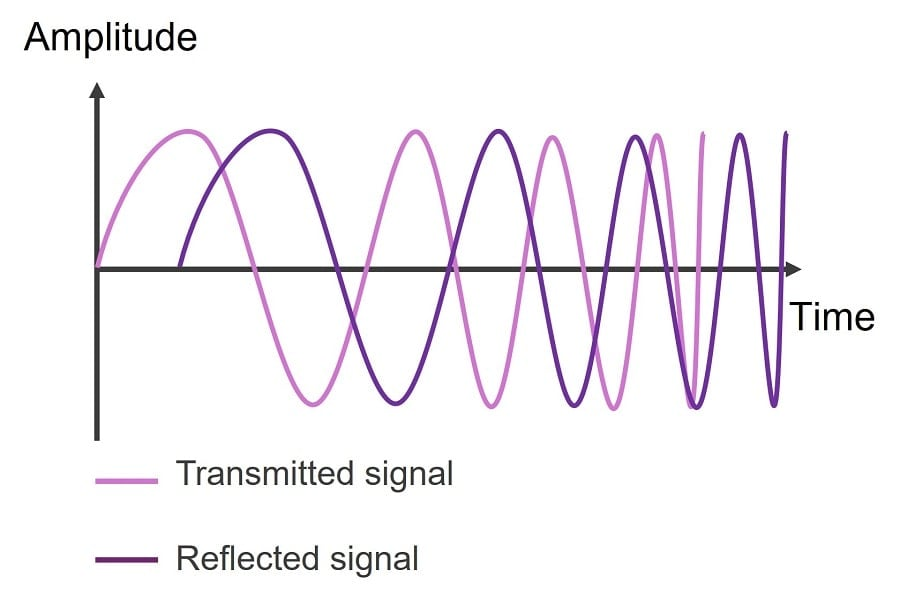
\includegraphics[scale=0.3]{pics/bab2/txRxWave.jpg}
		\caption[FMCW Dalam Domain Waktu]{FMCW Dalam Domain Waktu}
		\label{pic:FMCWTime}
	\end{center}
\end{figure}

Oleh karena itu, salah satu karakteristik dari radar FMCW adalah bahwa jarak pengukuran dapat dihitung dengan membandingkan frekuensi sinyal yang diterima dengan sinyal yang ditransmisikan.   

\begin{equation} 
	R = \frac{c \Delta{t}}{2} = \frac{c \Delta{f}}{2(\frac{d(f)}{d(t)})}
	\label{eq:PersFMCW}
\end{equation}

Persamaan \ref{eq:PersFMCW} menunjukkan jarak (R) dengan objek yang terdeteksi. Yang mana $\Delta{t}$ adalah waktu tunda dalam detik, $\Delta{f}$ merupakan pergeseran frekuensi terukur dalam Hertz, dengan d(f)/d(t) sebagai pergeseran frekuensi dalam suatu periode. 

\begin{equation}
	R_{max} = \frac{F_{s} c}{2 K}
	\label{eq:MaxRange}
\end{equation}

Persamaan \ref{eq:MaxRange} menunjukkan jarak maksimum yang dapat di deteksi oleh radar FMCW. $F_{s}$ merupakan frekuensi \textit{sampling}, dan K adalah tingkat kenaikan frekuensi pada suatu periode yang dapat dihitung dengan persamaan \ref{eq:slope} yaitu mengurangi nilai maksimum frekuensi dengan nilai minimumnya, lalu membaginya dengan waktu \textit{sweep} (\textit{chirp}).

\begin{equation}
	K = \frac{f_{atas} - f_{bawah}}{T_{c}}
	\label{eq:slope}
\end{equation}

Selain itu, salah satu faktor penting yang perlu diperhitungkan dalam perancangan radar FMCW adalah resolusi jarak. Resolusi jarak sendiri merupakan kemampuan dari suatu radar dalam membedakan dua buah objek yang berdekatan.

\begin{equation}
	\Delta{R} = \frac{c}{2 BW}
	\label{eq:RangeRes}
\end{equation}

Persamaan \ref{eq:RangeRes} menjelaskan bahwa dengan membagi kecepatan cahaya dengan dua kali lebar pita frekuensi (\textit{Bandwidth}), maka resolusi jarak akan didapatkan.

\subsection{\textit{Linear Frequency Modulated Continuous Wave Radar}}
\textit{Linear Frequency Modulated}, yang juga sering disingkat sebagai LFM adalah teknik pengolahan sinyal yang dilakukan dengan menyapu frekuensi dari bawah ke atas (\textit{Up-Chirp}) atau dari atas ke bawah (\textit{Down-Chirp}). Dengan $f_{0}$ sebagai frekuensi tengah, dan dilakukan pada \textit{bandwidth} yang telah ditentukan. Teknik ini akan membantu pencapaian radar dengan resolusi yang lebih tinggi karena \textit{bandwidth} yang dicapai akan menjadi lebih tinggi.

Salah satu jenis gelombang LFM adalah \textit{Linear Triangular Frequency Modulation} yang ditunjukkan pada gambar \ref{pic:LFMTriangular}. Penggunaan jenis gelombang tersebut akan mempermudah proses evaluasi target.

\begin{figure}
	\begin{center}
		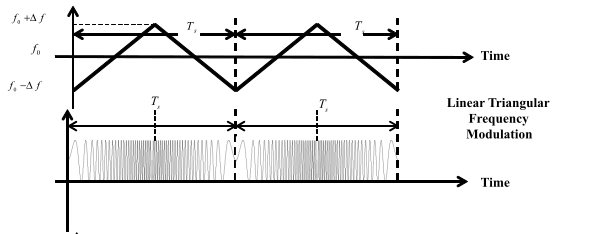
\includegraphics[scale=0.7]{pics/bab2/lfmTriangular.png}
		\caption[LFM Tipe Segitiga]{LFM Tipe Segitiga \cite{Jankiraman2018}}
		\label{pic:LFMTriangular}
	\end{center}
\end{figure}


Selain gelombang LFM segitiga, ada pula yang berbentuk seperti gigi gergaji (\textit{Sawtooth}) seperti gambar \ref{pic:lfmSaw}.

\begin{figure}
	\begin{center}
		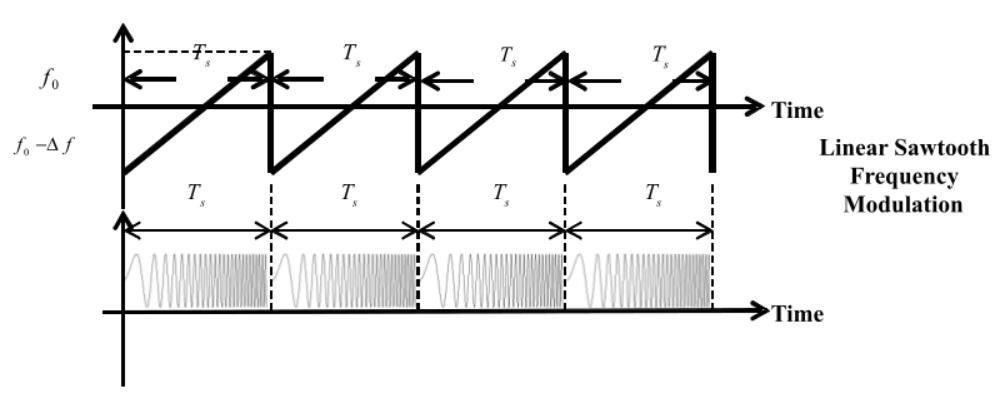
\includegraphics[scale=0.65]{pics/bab2/lfmSawtooth.png}
		\caption[LFM Tipe Gigi Gergaji]{LFM Tipe Gigi Gergaji \cite{Jankiraman2018}}
		\label{pic:lfmSaw}
	\end{center}
\end{figure}

Seluruh teknik tersebut memiliki keunggulannya masing masing. Keunggulan tersebut didapat karena proses analisis yang berbeda. Pada LFM berbentuk gigi gergaji, maka hanya objek diam saja yang dapat dideteksi jarak dan kecepatannya seperti pada gambar \ref{pic:lfmDetail}. Namun bila menggunakan LFM berbentuk segitiga, maka objek yang bergerak dapat dideteksi jarak dan kecepatannya dalam waktu yang bersamaan.

\begin{figure}
	\begin{center}
		\includegraphics[scale=0.65]{pics/bab2/lfmDetail.png}
		\caption[Detail Analisis LFM \textit{Sawtooth}]{Detail Analisis LFM \textit{Sawtooth} \cite{Jankiraman2018}}
		\label{pic:lfmDetail}
	\end{center}
\end{figure}


\subsection{Teknik Pengolahan Sinyal}
Untuk melakukan pengambilan keputusan dari data yang diambil oleh radar, maka dibutuhkan langkah pengolahan yang benar dan mencakup berbagai hal. Beberapa parameter yang bisa diambil estimasinya adalah jarak dan kecepatan dari objek yang terdeteksi. Pada estimasi jarak, persamaan \ref{eq:RangeEst} dapat menjelaskan hubungan jarak dengan beberapa faktor yang mempengaruhinya.

\begin{equation}
	d_{0} = \frac{c f_{b}}{2 \mu} = \frac{c T_{c} f_{b}}{2 B}
	\label{eq:RangeEst}
\end{equation}

Pada persamaan tersebut, terdapat c sebagai kecepatan cahaya, $f_{b}$ adalah \textit{beat frequency} yang merupakan perbedaan pada frekuensi,  $\mu$ yang merupakan laju perubahan frekuensi pada suatu waktu (\textit{chirp rate}), dengan $T_{c}$ sebagai waktu \textit{Sweep}. Sedangkan untuk melakukan estimasi kecepatan terdapat pergeseran frekuensi akibat efek doppler, yang menjelaskan perubahan frekuensi suatu gelombang karena suatu objek sumber yang bergerak. Bila pergeseran doppler ($f_{d}$), dengan v sebagai kecepatan, dan $\lambda$ adalah panjang gelombang, maka didapatkan persamaan \ref{eq:velocity}.

\begin{equation}
	v = \frac{f_{d}}{2}\lambda
	\label{eq:velocity}
\end{equation}

\subsection{Perhitungan \textit{Error}}
Penghitungan galat dari radar yang telah didesain dapat dilakukan dengan menguji keakurasian dari hasil deteksi. Hasil akurasi deteksi radar dapat diuji dengan menggunakan \textit{Root Mean Square Error} (RMS E) dari \textit{Signal to Noise Ratio}, sesuai persamaan \ref{eq:sigmaRN}.

\begin{equation}
	\sigma_{RN} = \frac{RMS E}{\sqrt{2 SNR_{L}}}
	\label{eq:sigmaRN}
\end{equation}

Dengan nilai dari RMS E bisa didapat dengan persamaan \ref{eq:rmsE}.

\begin{equation}
	RMS E = \frac{\sqrt{\sum_{t = 1}^{k} (m(t)-n(t))^2}}{k}
	\label{eq:rmsE}
\end{equation}

Nilai dari k adalah jumlah data, dengan m sebagai hasil data berdasarkan simulasi, dan n adalah data sebenarnya. Dengan begitu, nilai akurasi deteksi radar dapat dihitung dengan persamaan \ref{eq:accRadar}.

\begin{equation}
	Akurasi = 1 - \sigma_{RN}
	\label{eq:accRadar}
\end{equation}

\section{\textit{Software Defined Radio}}
\textit{Software Defined Radio} atau yang sering disingkat menjadi SDR merupakan teknologi komunikasi berbasis nirkabel yang kegunaannya dapat ditentukan oleh perangkat lunak \cite{Anisah2018}. Sehingga dalam implementasinya, tidak perlu dilakukan perubahan perangkat keras baru bila ingin melakukan perubahan, baik dari segi standar, teknologi, dan layanan. Hanya dengan melakukan perubahan konfigurasi saja, lalu SDR akan langsung dapat digunakan. 

Dalam implementasinya, SDR membutuhkan \textit{Universal Software Radio Peripheral}, atau yang sering disingkat menjadi USRP merupakan \textit{hardware} yang merupakan bagian \textit{front end} pada arsitektur sistem SDR. USRP terdiri dari modul yang dapat terkoneksi dengan komputer sehingga memperbolehkan pemrograman dengan aplikasi seperti GNURadio dan LabVIEW \cite{Gulo2023}. 

Penggunaan USRP sangat memudahkan proses perancangan prototipe dan pengujian karena adanya antarmuka yang dapat mengkoneksikan USRP dengan antena dan berbagai macam bagian perangkat keras yang dibutuhkan.

\subsection{\textit{Universal Software Radio Peripheral}}

\textit{Universal Software Radio Peripheral} atau yang sering disingkat dengan USRP merupakan \textit{platform} yang digunakan dalam mengimplementasikan SDR. Di dalam USRP terdapat \textit{Field Programmable Gate Array} atau FPGA yang merupakan suatu \textit{Integrated Circuit} yang dapat diprogram. Pada hal ini, USRP adalah perangkat keras yang dapat menerima dan mentransmisikan gelombang radio.

Kemampuannya untuk berinteraksi dengan gelombang radio inilah, ditambah pula dengan kemudahannya untuk melakukan pemrograman terhadap USRP ini yang membuat alat ini terkenal di kalangan akademisi dan peneliti. Karena pelaksanaan dan pengembangan prototipe menjadi lebih mudah dengan menghapuskan keperluan pengadaan komponen dalam prototipe.

\begin{center}
	\begin{figure}[h!]
		\begin{subfigure}[b]{0.5\linewidth}
			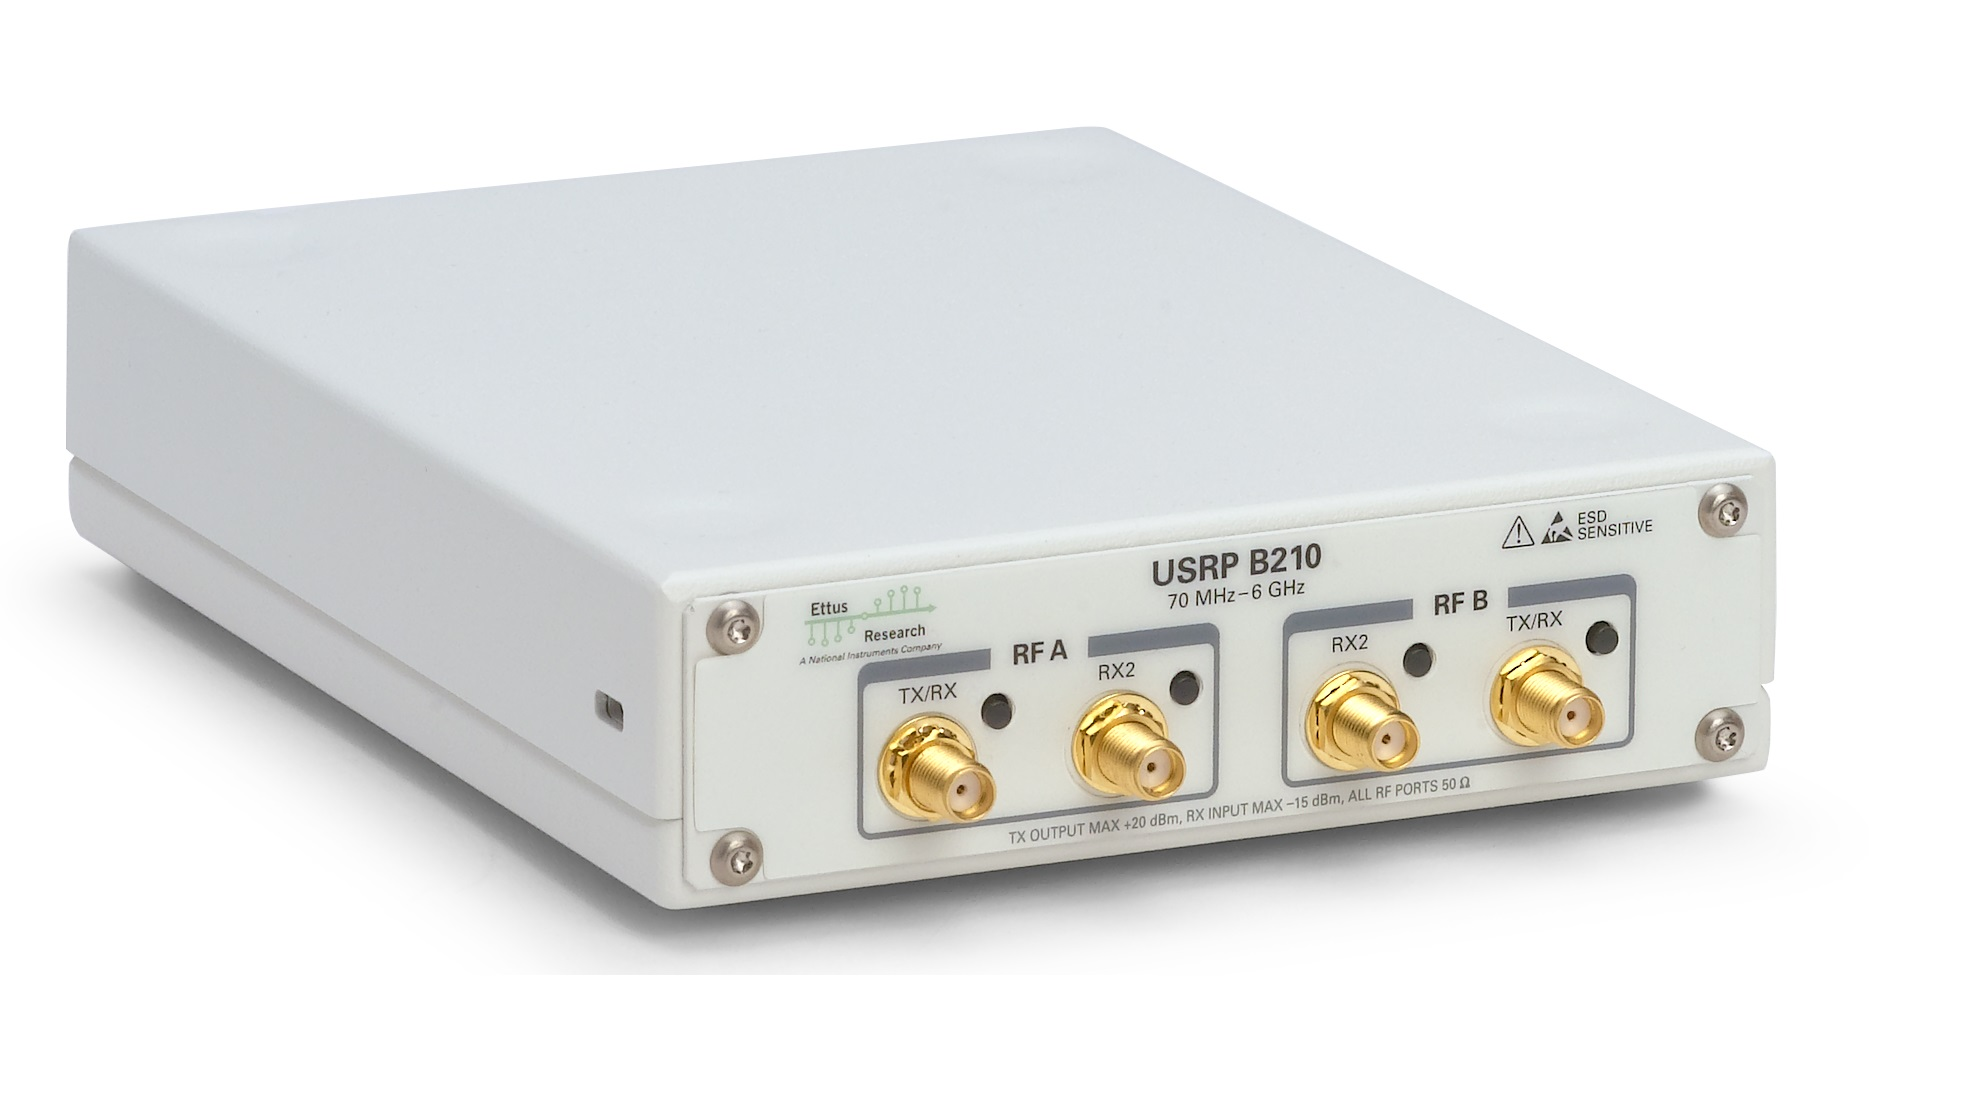
\includegraphics[width=\linewidth]{pics/bab2/B210.jpg}
			\caption{USRP B210 dengan \textit{enclosure}}
		\end{subfigure}
		\begin{subfigure}[b]{0.5\linewidth}
			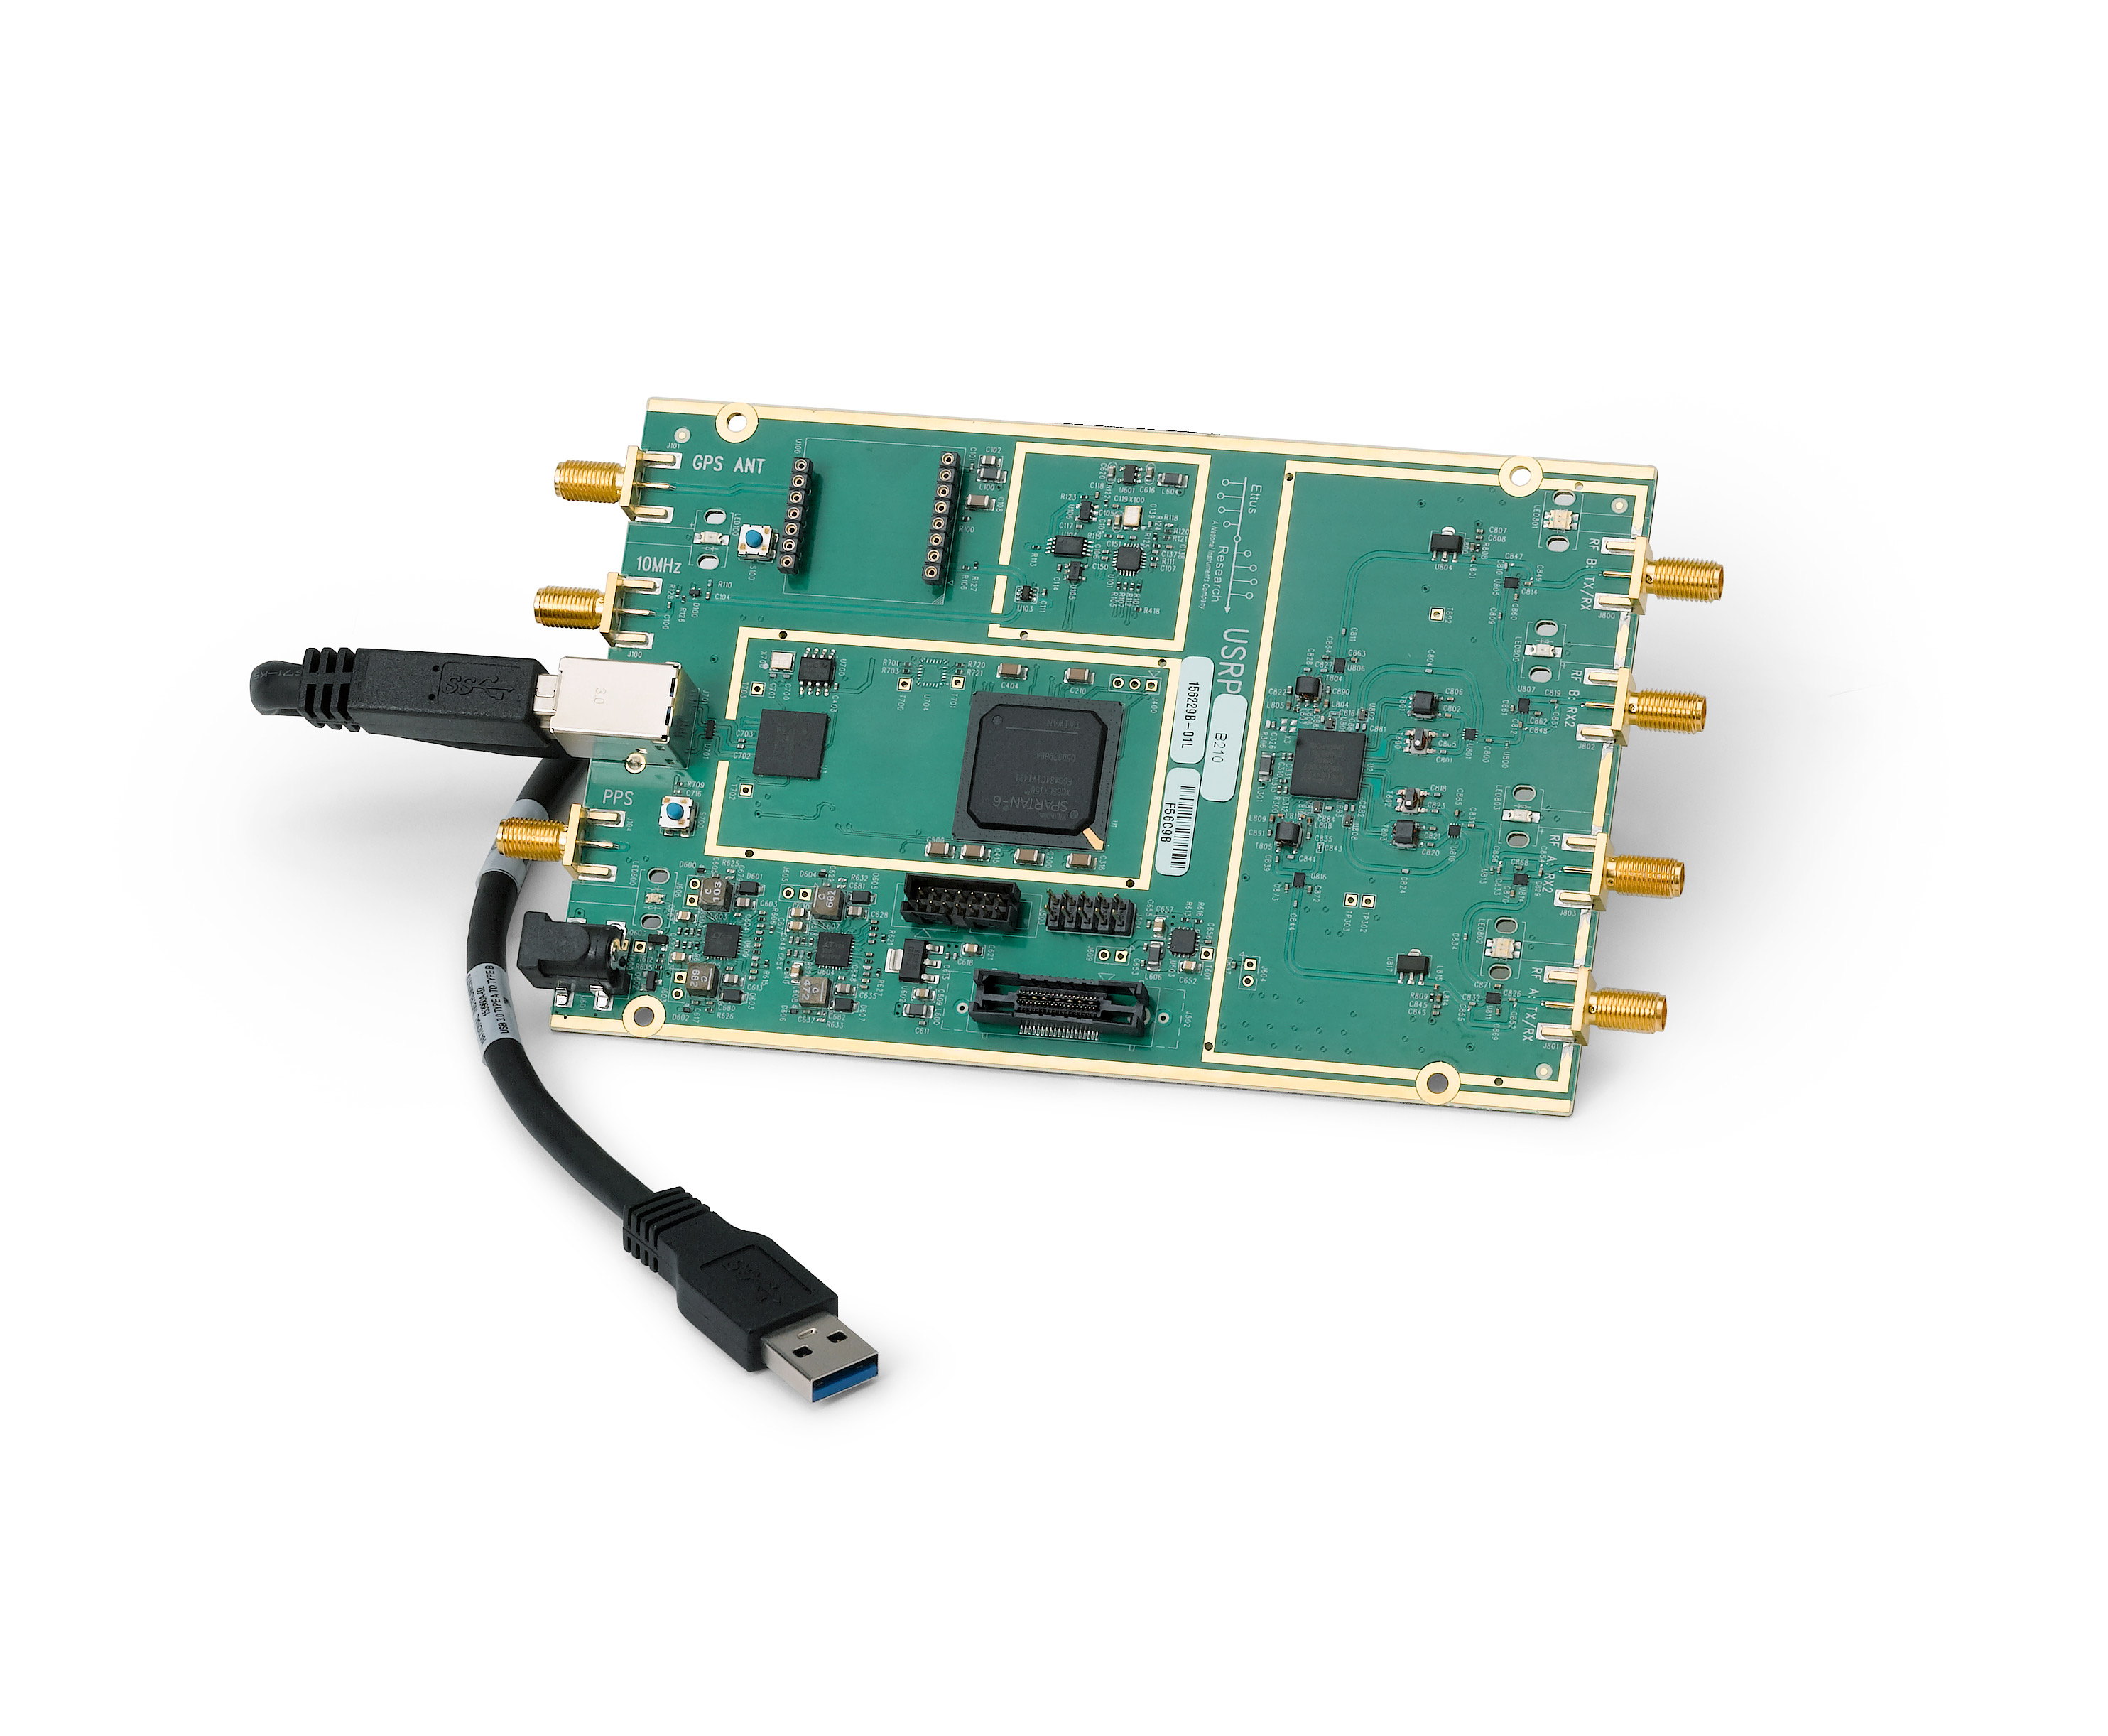
\includegraphics[width=7.3cm]{pics/bab2/B210Board.jpg}
			\caption{\textit{Board} USRP B210}
		\end{subfigure}
		\caption{USRP B210}
		\label{pic:gambarusrp}
	\end{figure}
\end{center}

Ada beberapa USRP yang ada di pasar, salah satu yang cukup seringkali digunakan adalah USRP buatan dari \textit{Ettus}. Salah satu serinya adalah B210 seperti pada gambar \ref{pic:gambarusrp}. Penggunaan seri ini tidak tanpa alasan, karena seperti yang dapat dilihat pada tabel \ref{tab:spekb210}, spesifikasi USRP ini cukup memenuhi kebutuhan riset pada frekuensi yang sering di gunakan, dengan kapabilitas pengolahan sampel yang baik.

\begin{longtable}{|c|c|c|c|}
	\caption{Spesifikasi \textit{USRP} B210}
	\label{tab:spekb210}\\
	\hline
	No. & Keterangan & Nilai & Satuan \\
	\hline
	1. & \textit{RF Coverage} & 70 - 6 & MHz - GHz \\
	\hline
	2. & \textit{Analog to Digital Converter Sample Rate} (maksimum) & 61.44 & MS/s \\
	\hline
	3. & \textit{Analog to Digital Resolution}  & 12 & bits	\\
	\hline
	4. &\textit{Analog to Digital Wideband SFDR} & 78 & dBc \\
	\hline
	5. & \textit{Digital to Analog Converter Sample Rate} (maksimum) & 61.44 & MS/s \\
	\hline
	6. & \textit{Digital to Analog Resolution}  & 12 & bits	\\
	\hline
	7. & \textit{Host Sample Rate} (16b) & 61.44 & MS/s \\
	\hline
	8. & \textit{Frequency Accuracy} & $\pm 2.0$ & ppm \\
	\hline
	9. &  \textit{W/ GPS Unlocked TCXO Reference} & $\pm 75$ & ppb \\
	\hline
	10. & \textit{W/ GPS Locked TCXO Reference} & $<$ 1 & ppb \\ 
	\hline
\end{longtable}

Dengan spesifikasi tersebut, maka USRP B210 memiliki kemampuan \textit{instantneous bandwidth} hingga 56 MHz pada transmisi 1 X 1 dan 30.72 MHz pada transmisi 2 X 2.

\subsection{\textit{GNURadio}}

\begin{figure}
	\begin{center}
		
\includegraphics[scale=0.5]{pics/bab2/GNU.png} 
		\caption[Logo GNURadio]{Logo GNURadio}
		\label{pic:logoGnuRadio}
	\end{center}
\end{figure}
GNURadio adalah aplikasi yang dapat melakukan pemrograman terhadap USRP lewat antarmuka. GNURadio merupakan \textit{software open source} sehingga semua orang dapat mengakses, mengubah, dan membagikan \textit{source code} dari program tersebut secara bebas. Dengan menggunakan aplikasi ini, perubahan parameter pada USRP dapat dilakukan dengan mudah.

\begin{figure}
	\begin{center}
		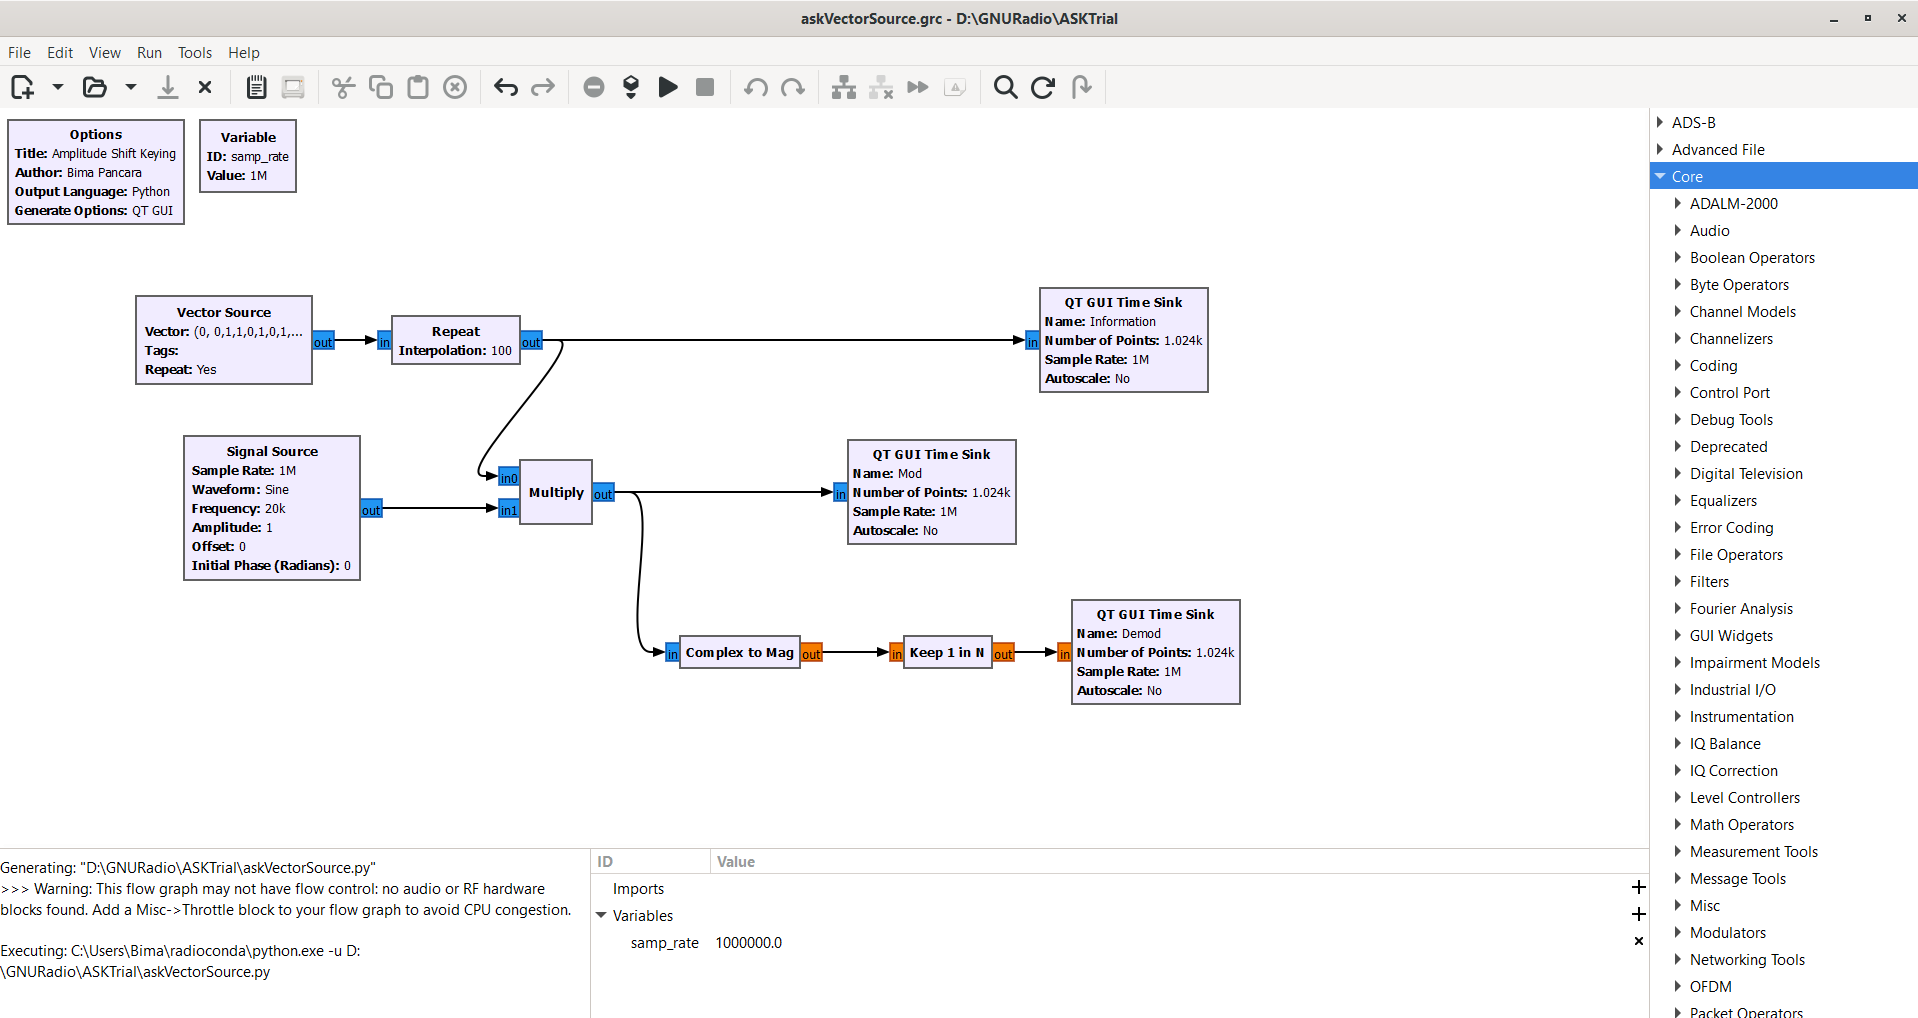
\includegraphics[scale=0.35]{pics/bab2/blokDiagramGRC.png} 
		\caption[Contoh \textit{Flowgraph} GNURadio]{Contoh \textit{Flowgraph} GNURadio}
		\label{pic:contohBlokGRC}
	\end{center}
\end{figure}

Gambar \ref{pic:contohBlokGRC} adalah contoh blok diagram sistem (\textit{flowgraph}) yang sukses dibuat pada aplikasi GNURadio. Pada gambar \ref{pic:contohRunGRC} menunjukkan hasil bila desain sistem tersebut dijalankan.

\begin{figure}
	\begin{center}
		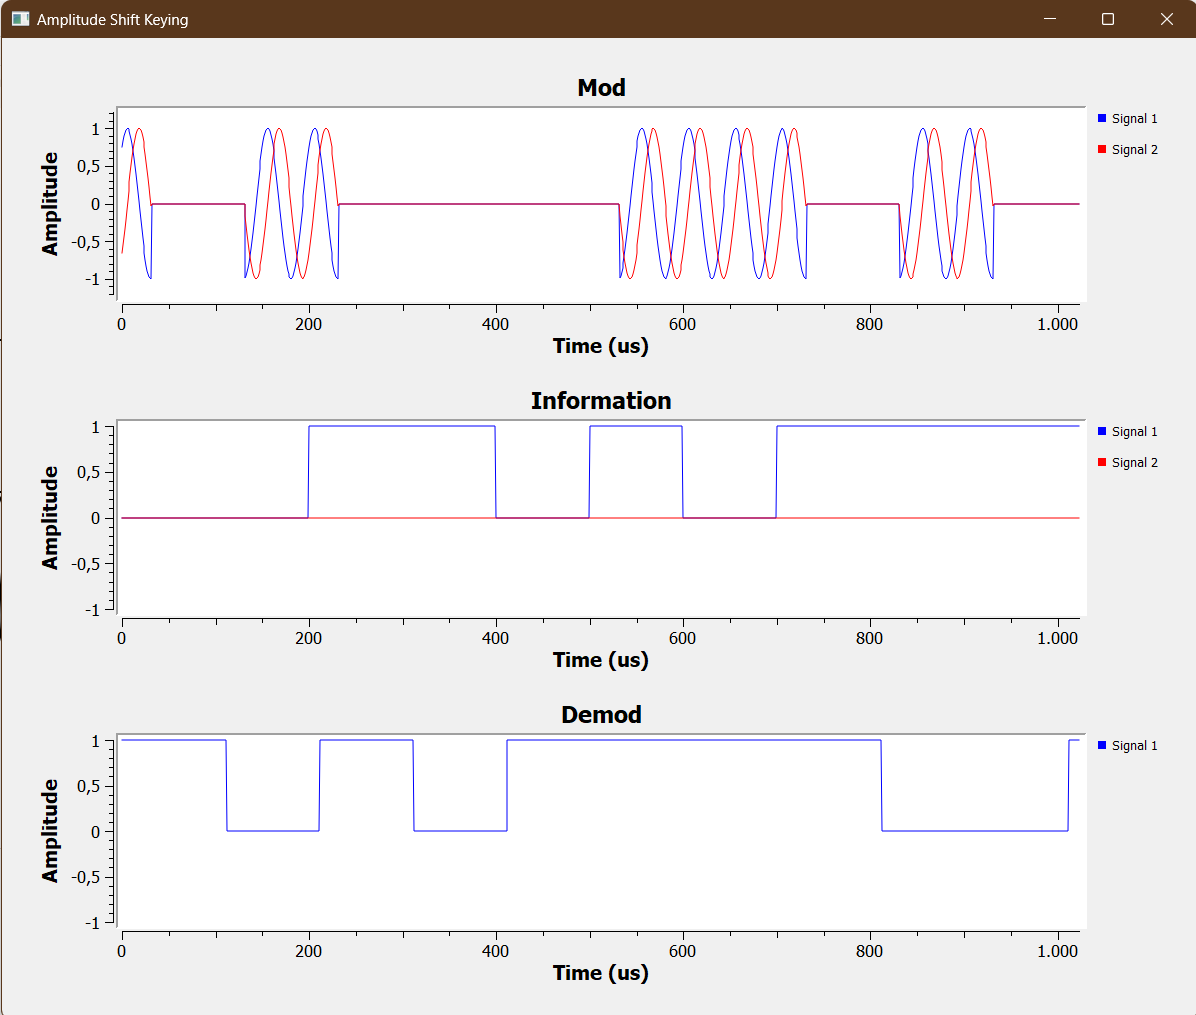
\includegraphics[scale=0.4]{pics/bab2/contohRunGRC.png} 
		\caption[Hasil Desain Sistem GNURadio]{Hasil Desain Sistem GNURadio}
		\label{pic:contohRunGRC}
	\end{center}
\end{figure}



